\documentclass{article}
\usepackage{fancyhdr}
\usepackage{graphicx}
\usepackage{amsmath}
\usepackage{xcolor}
\usepackage[margin=1in]{geometry}

\pagestyle{fancy}
\graphicspath{ {./img/} }

\begin{document}
	\begin{titlepage}
		\begin{center}
			\vspace{1cm}
			{\LARGE\textbf{Programming the Microarchitecture Design}}

			\vspace{1.5cm}
			\textbf{\large Ghassan Arnouk}\\
			
			\vspace{1cm}
			\large SYSC 3006A\\
			\large Summer 2020\\
			\large Lab 4 Report\\
			\large Group 1\\
			
						
			\vspace{2cm}
			\textbf{Instructor:} Michel Sayde\\
			
			\vspace{0.1cm}
			\textbf{TA:} Khalid Almahrog\\
			
			\vspace{0.1cm}
			\textbf{Submitted:} 2020/06/05\\			
		\end{center}
	\end{titlepage}
	
	\lhead{Ghassan Arnouk (Group 1)}
	\rhead{Programming the Microarchitecture Design}
	\pagebreak
	
	\section{First Part}
	\subsection{Control FSM Output Table}
	\subsubsection {Complete the provided Control FSM Output Table for Part 1 for the Fetch, Decode, and Execution States for opcodes 0x01 (ADD) through 0x07 (NOT).}
	\begin{table}[!ht]
		\centering
		\caption{Fetch, Decode, and Execution States for opcodes 0x01 (ADD) through 0x07 (NOT)}
		\vspace{0.2cm}
		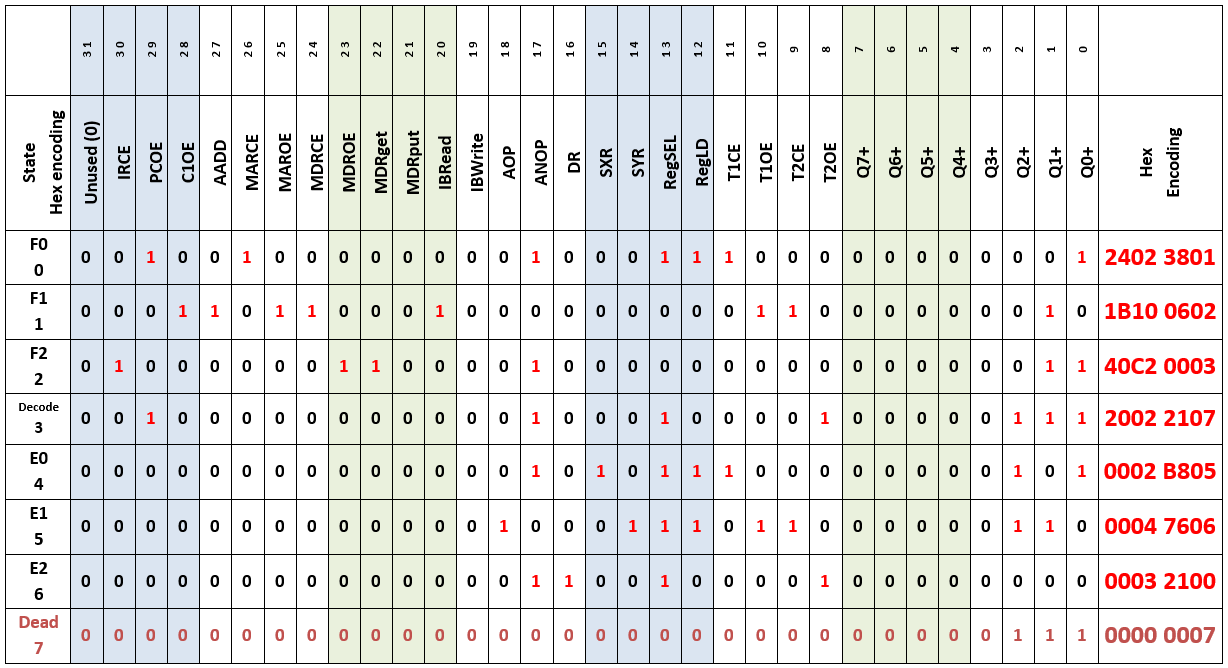
\includegraphics[width=\linewidth]{fetch_decode_executionStates.png}		

	\end{table}
	
	\pagebreak
	
	\section{Second Part}
	\subsection {Control FSM Output Table}
	\subsubsection{Complete the provided Control FSM Output Table for Part 2 for NOP Instruction Execution 3 States. This table will extend the Control FSM Output Table for Part 1 (same FSM Output ROM).}
	\begin{table}[!ht]
		\centering
		\caption{NOP Instruction Execution States}
		\vspace{0.2cm}
		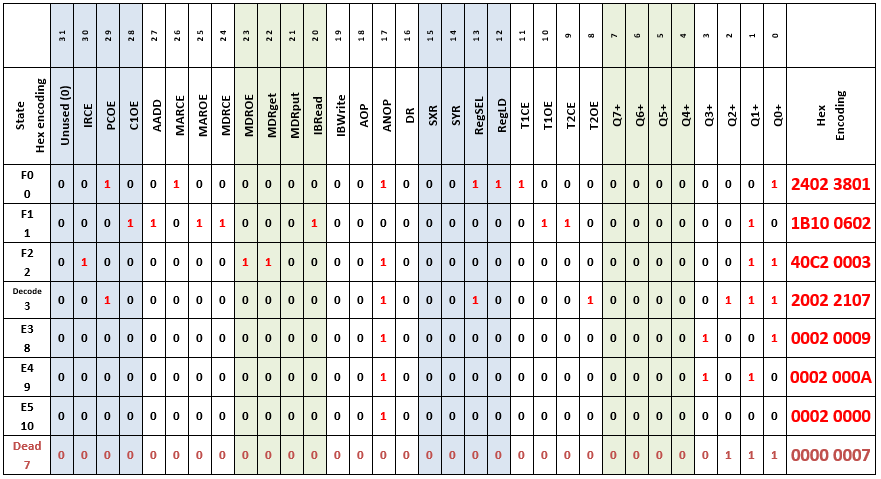
\includegraphics[width=\linewidth]{nop_instruction.png}
	\end{table}

	\pagebreak
	
	\section{Third Part}
	\subsection{Control FSM Output Table}
	\subsubsection{Complete the provided Control FSM Output Table for Part 3 for NEG Instruction Execution States. This table will extend the Control FSM Output Table for Part 1 and 2 (same FSM Output ROM).}
	\begin{table}[!ht]
		\centering
		\caption{NEG Instruction Execution States}
		\vspace{0.2cm}
		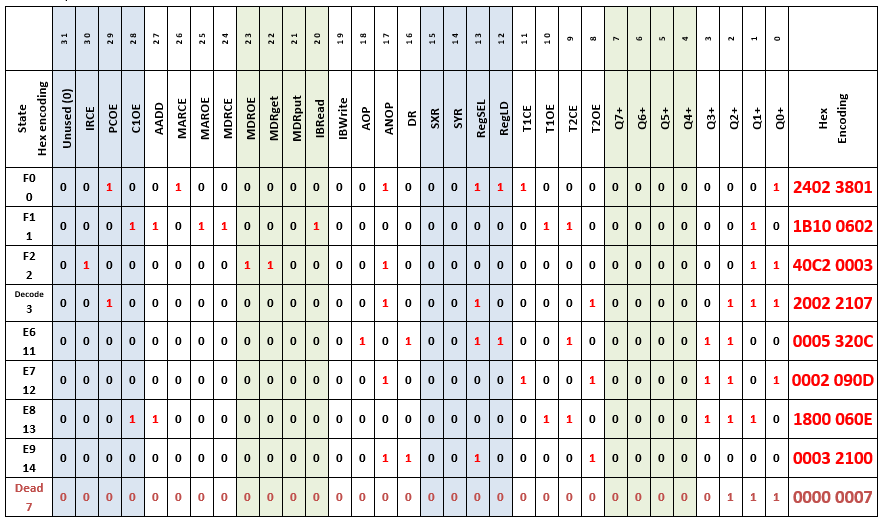
\includegraphics[width=\linewidth]{neg_instruction.png}
	\end{table}

	\subsection{Describe how NEG instruction is executed at each execution state.}
	NEG can be performed by initially doing a NOT operation in the ALU and then adding a 1 to it.
	The 1 is the constant received from C1OE.
	The add operation is similar to  incrementing the PC in previous labs.
	The Opcode for the NEG operation is 0x17 while it is 0x00 for the NOP operation.
	
	\pagebreak
	
	\subsection{Decode ROM Table}
	\subsubsection{Complete the provided FSM Decode ROM Table to show any entries that must be programmed (for all parts).}
	\begin{table}[!ht]
		\centering
		\caption{FSM Decode ROM Table}
		\vspace{0.2cm}
		\begin{tabular}{|c|c|c|}
			\hline
			Instruction & Address (Hex) & Contents (Hex)\\
			\hline\hline
			NOP & 00 & \textcolor{red}{08}\\
			\hline
			ADD & 01 & 04\\
			\hline
			SUB & 02 & 04\\
			\hline
			MOV & 03 & 05\\
			\hline
			AND & 04 & 04\\
			\hline
			OR & 05 & 04\\
			\hline
			XOR & 06 & 04\\
			\hline
			NOT & 07 & 05\\
			\hline
			NEG & \textcolor{red}{17} & \textcolor{red}{0B}\\
			\hline
		\end{tabular}
	\end{table}

	\section{Fourth Part}
	\subsection{Instruction Table}
	\subsubsection{Complete the provided Main Memory Table to contain the encodings of the Test Program instructions as indicated. Then program the words of this table into the Main Memory. Be sure to include the Main Memory contents exactly as given in the table.}
	
	\begin{table}[!ht]
		\centering
		\caption{Main Memory Table}
		\vspace{0.2cm}
		\begin{tabular}{|c|c|c|}
			\hline
			Address (Hex) & Instruction (Hex) & Encoding (Hex)\\
			\hline\hline
			0 & R2 $\leftarrow$ [R15] & 0320 F000\\
			\hline
			1 & R11 $\leftarrow$ NOT [R2] & 07B0 2000\\
			\hline
			2 & R10 $\leftarrow$ [R15] & 03A0 F000\\
			\hline
			3 & R15 $\leftarrow$ [R10] - R[11] & 02FA B000\\
			\hline
			4 & EEBB FFFF & illegal instruction\\
			\hline
			5 & NOP & 0000 0000\\
			\hline
			6 & R11 $\leftarrow$ -[R11] & 17B0 0000\\
			\hline
		\end{tabular}
	\end{table}

	\pagebreak

	\subsection{Test Results}
	\subsubsection{Cycle the System Clock through the execution of your Test program and show your logs here.}
	\begin{table}[!ht]
		\centering
		\caption{Simulation Log of the Circuit}
		\vspace{0.2cm}
		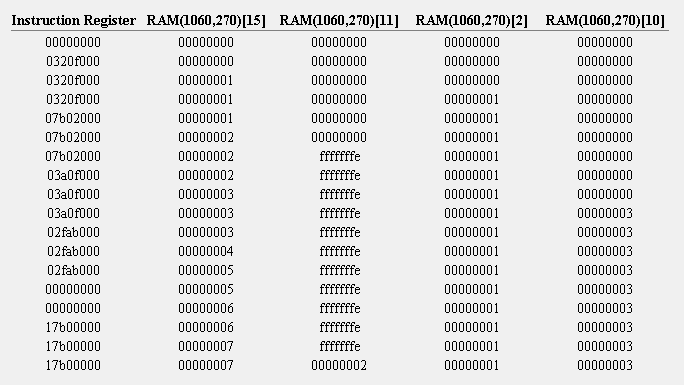
\includegraphics[width=\linewidth]{sim_log_table.png}
	\end{table}
\end{document}